\subsection{An experiment with bacteria}

\begin{frame}{Experiments}
    
\end{frame}

\subsection{An experiment with cells}

\begin{frame}{Tumor-Stroma Interactions}

    \begin{itemize}
        \item \textbf{Title:} Evolutionary Dynamics of Tumor-Stroma Interactions in Multiple Myeloma.
        \item \textbf{Authors:} Javad Salimi Sartakhti, Mohammad Hossein Manshaei, Soroosh Bateni, Marco Archetti.
        \item Cancer cells and stromal cells cooperate by exchanging diffusible factors.
        \begin{itemize}
            \item Frequency-dependent selection that can be studied in the framework of evolutionary game theory.
        \end{itemize}
    \end{itemize}
    
\end{frame}

\begin{frame}{Tumour-Stroma Interactions: payoff functions}
    \begin{itemize}
        \item There are $n$ phenotypes in a population denoted by $\{ P_1, \ldots, P_n \}$.
        \item Each phenotype can produce one diffusible factor $\{ G_1, \ldots, G_n \}$.
        \item Each diffusible factor $j$ has a different effect $r_{i,j}$ on the other phenotypes $i$.
        \item The cost for $P_i$ for growth factor $G_i$ is denoted as $c_i$.
        \item $M$ is the number of cells within the diffusion range.
        \begin{itemize}
            \item There are $M_j$ individuals of type $P_j$ among the other group members.
        \end{itemize}
        \item The payoff for strategy $P_j$ is:
        \begin{align*}
            \pi_{P_j}(M_1,\ldots,M_n)=\frac{(M_j+1)\times c_j}{M}r_{j,j} + \sum_{i=1, i \neq j}^n \frac{M_i \times c_i}{M}r_{j,i} - c_j \;.
        \end{align*}
    \end{itemize}
\end{frame}

\begin{frame}{Tumour-Stroma Interactions: dynamics}
    \begin{columns}
        \begin{column}{0.4\textwidth}
             \begin{itemize}
                \item Malignant plasma cells.
                \item Osteoblasts.
                \item Osteoclasts.
                \item Growth factors:
                \begin{itemize}
                    \item Autocrine effects.
                    \item Paracrine effects. 
                \end{itemize}
            \end{itemize}
        \end{column}
        \begin{column}{0.6 \textwidth}
            \begin{figure}[t]
                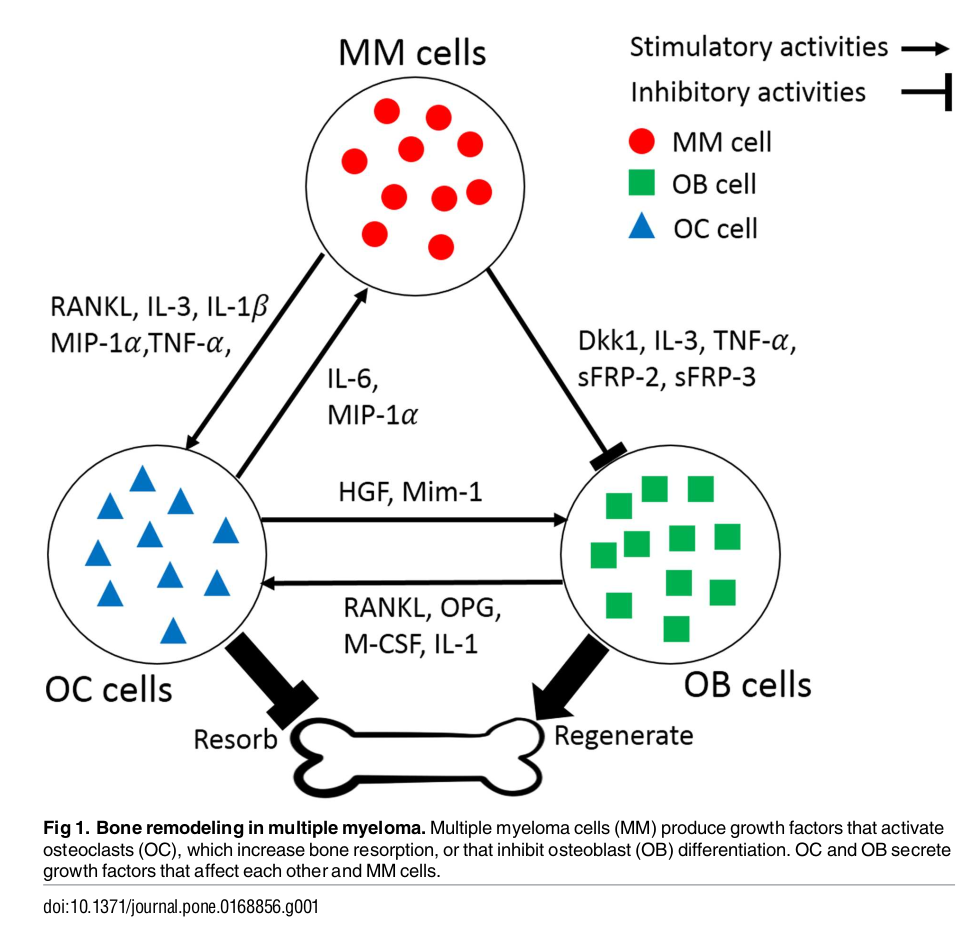
\includegraphics[width=0.9\linewidth]{img/tumour_stroma_interactions.png}
            \end{figure}
        \end{column}
    \end{columns}
\end{frame}



\begin{frame}{Tumour-Stroma Interactions: Scenario 1}
    \begin{itemize}
        \item $c_1<c_2<c_3$ (a common occurrence in multiple myeloma).
        \item In the presence of a small number of MM cells, the stable point on the OB-OC border becomes a saddle point and clonal selection leads to a stable coexistence of OC and MM cells.
    \end{itemize}
    
    \begin{columns}
        \begin{column}{0.4\textwidth}
            \begin{figure}[t]
                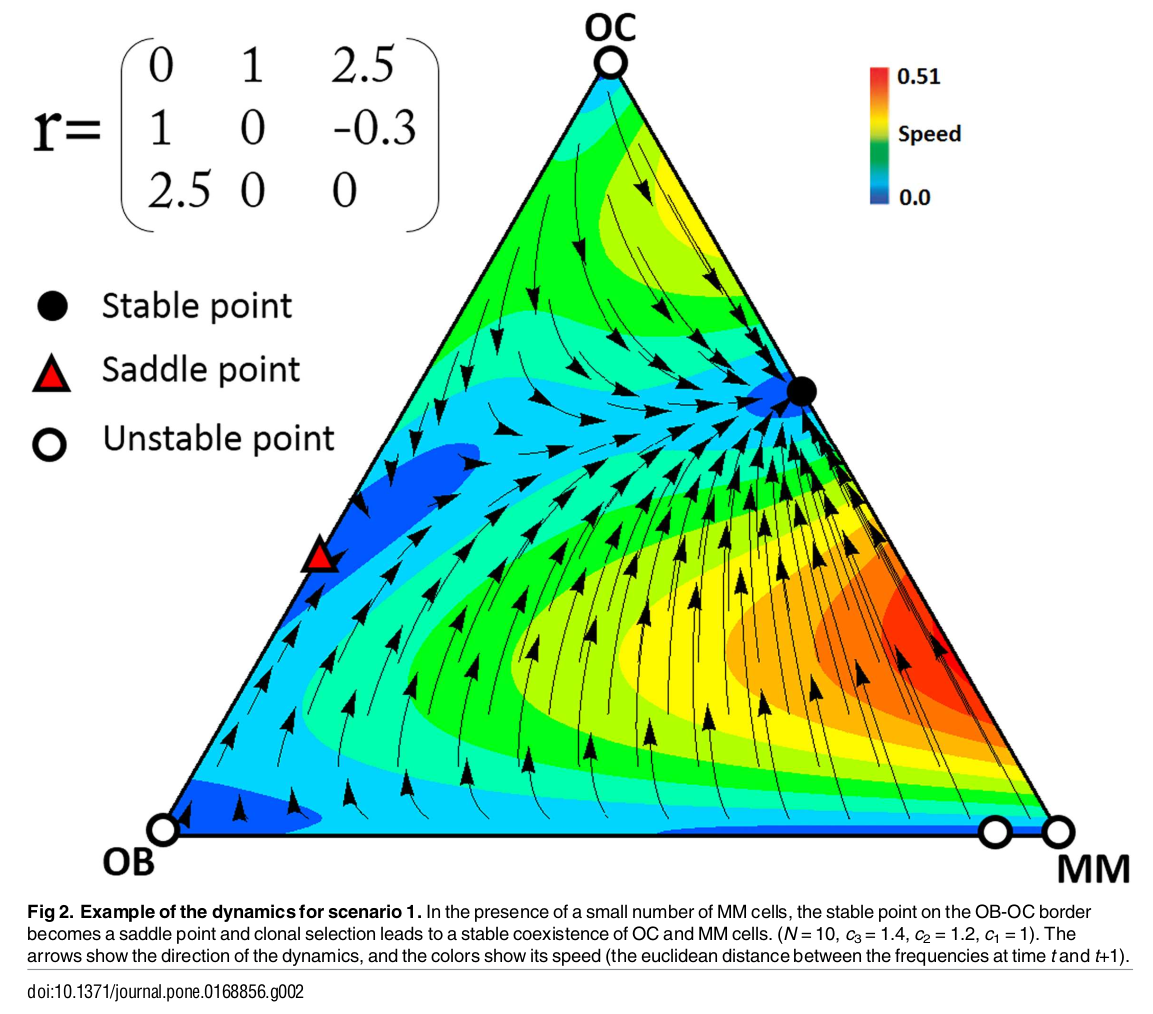
\includegraphics[width=0.9\linewidth]{img/Scenario1.png}
            \end{figure}
        \end{column}
        \begin{column}{0.6\textwidth}
            \begin{figure}[t]
                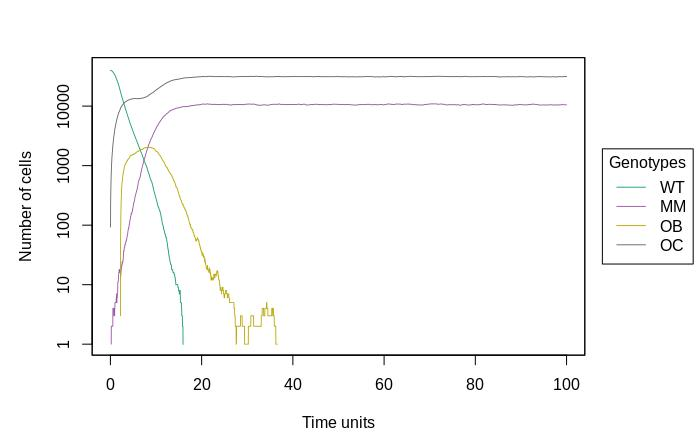
\includegraphics[width=0.9\linewidth]{img/scenario1_tr.jpg}
            \end{figure}
        \end{column}
    \end{columns}
\end{frame}

\begin{frame}{Tumour-Stroma Interactions: Scenario 2}
    \begin{itemize}
        \item $c_1=c_2=c_3$.
        \item The game has one polymorphic stable point between OB and OC. In this case, clonal selection leads to the regular OC-OB balance and prevents invasion of MM cells.
    \end{itemize}
    
    \begin{columns}
        \begin{column}{0.4\textwidth}
            \begin{figure}[t]
                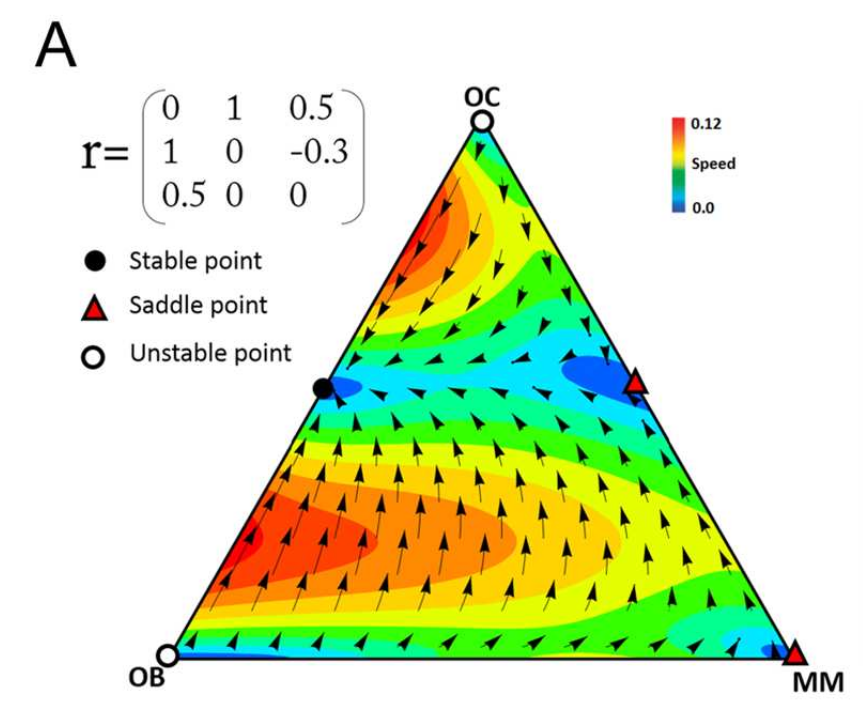
\includegraphics[width=0.9\linewidth]{img/Scenario2.png}
            \end{figure}
        \end{column}
        \begin{column}{0.6\textwidth}
            \begin{figure}[t]
                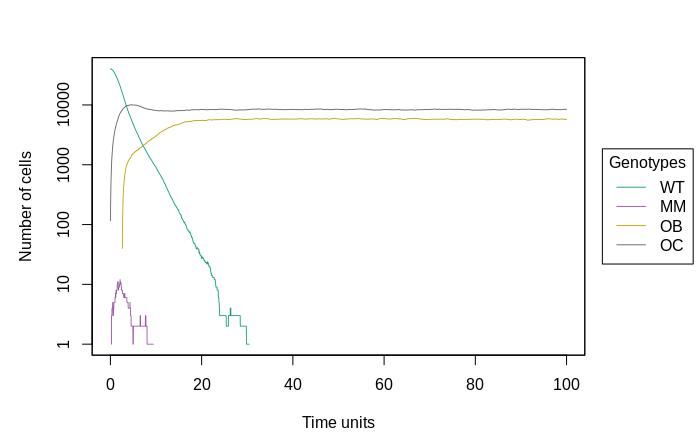
\includegraphics[width=0.9\linewidth]{img/scenario2_tr.jpg}
            \end{figure}
        \end{column}
    \end{columns}
\end{frame}